\documentclass[aspectratio=169]{beamer}
\usetheme{Madrid}
\usecolortheme{default}
\usepackage{booktabs}
\usepackage{graphicx}
\usepackage{tikz}
\usetikzlibrary{arrows.meta, positioning}

\definecolor{accent}{RGB}{0, 102, 153}
\setbeamercolor{title}{fg=white, bg=accent}
\setbeamercolor{frametitle}{fg=white, bg=accent}
\setbeamercolor{structure}{fg=accent}

\title[LLM Smart Contract Security]{From Prompt to Exploit:\\Security Vulnerabilities in LLM-Generated Smart Contracts}
\subtitle{CSC 5991 --- Introduction to LLM: Project Proposal}
\author{Anonymous Author(s)}
\institute{Anonymous Institution}
\date{March 2026}

\begin{document}

%--- Slide 1: Title ---
\begin{frame}
\titlepage
\end{frame}

%--- Slide 2: Motivation ---
\begin{frame}{Why This Matters}
\begin{columns}
\begin{column}{0.55\textwidth}
\begin{itemize}
    \item Developers today often use tools like ChatGPT and Copilot to write smart contracts in Solidity
    \item These contracts handle real money --- sometimes billions of dollars in DeFi protocols
    \item The catch: once you deploy a smart contract, you \textbf{can't patch it}. Bugs stay forever
    \item So we wanted to ask a simple question: \textbf{how safe is the code that LLMs actually produce?}
\end{itemize}
\end{column}
\begin{column}{0.4\textwidth}
\centering
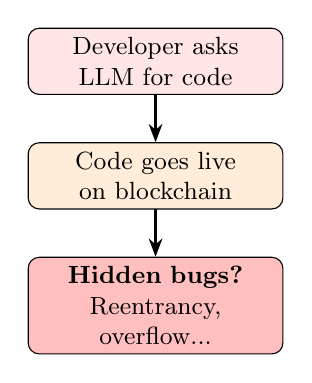
\begin{tikzpicture}[scale=0.85]
    \node[draw, rounded corners, fill=red!10, text width=3cm, align=center, font=\small] (llm) {Developer asks\\LLM for code};
    \node[draw, rounded corners, fill=orange!15, text width=3cm, align=center, font=\small, below=0.6cm of llm] (deploy) {Code goes live\\on blockchain};
    \node[draw, rounded corners, fill=red!25, text width=3cm, align=center, font=\small, below=0.6cm of deploy] (vuln) {\textbf{Hidden bugs?}\\Reentrancy, overflow...};
    \draw[-{Stealth}, thick] (llm) -- (deploy);
    \draw[-{Stealth}, thick] (deploy) -- (vuln);
\end{tikzpicture}
\end{column}
\end{columns}
\end{frame}

%--- Slide 3: What We Want to Find Out ---
\begin{frame}{What We Want to Find Out}
\begin{enumerate}
    \item[\textbf{RQ1.}] How common are security bugs in contracts that LLMs generate?
    \vspace{0.3cm}
    \item[\textbf{RQ2.}] Are some LLMs better or worse than others at writing safe code?
    \vspace{0.3cm}
    \item[\textbf{RQ3.}] What kinds of bugs show up the most?
    \vspace{0.3cm}
    \item[\textbf{RQ4.}] Can we trick LLMs into writing even more vulnerable code with sneaky prompts?
    \vspace{0.3cm}
    \item[\textbf{RQ5.}] Does the type of contract matter? (e.g., a simple token vs.\ a complex bridge)
    \vspace{0.3cm}
    \item[\textbf{RQ6.}] Are there any bug patterns that are unique to LLM-written code?
\end{enumerate}
\end{frame}

%--- Slide 4: Our Approach ---
\begin{frame}{Our Approach}
\begin{columns}
\begin{column}{0.55\textwidth}
\begin{enumerate}
    \item \textbf{Design prompts} --- we wrote 300 prompts covering 20 types of smart contracts (tokens, DeFi, bridges, governance, etc.)
    \vspace{0.15cm}
    \item \textbf{Generate contracts} --- we feed those prompts to 8 different LLMs and collect the Solidity code they produce (2,400 contracts total)
    \vspace{0.15cm}
    \item \textbf{Scan for vulnerabilities} --- we run three industry-standard security tools (Slither, Mythril, Semgrep) on every contract
    \vspace{0.15cm}
    \item \textbf{Test adversarial prompts} --- we also try prompts designed to trick the LLM into writing unsafe code, and compare
    \vspace{0.15cm}
    \item \textbf{Statistical analysis} --- we use non-parametric tests to compare across LLMs, categories, and prompt types
\end{enumerate}
\end{column}
\begin{column}{0.42\textwidth}
\footnotesize
\textbf{8 LLMs we are testing:}
\begin{itemize}
    \item GPT-4o (OpenAI)
    \item GPT-5 (OpenAI)
    \item Claude 3.5 Sonnet (Anthropic)
    \item Gemini 2.5 Flash-Lite (Google)
    \item DeepSeek Coder V2
    \item Qwen 2.5 Coder 32B
    \item CodeLlama-34B (Meta)
    \item Codestral 22B (Mistral)
\end{itemize}
\vspace{0.3cm}
\textbf{3 security tools:}
\begin{itemize}
    \item Slither --- fast static analysis
    \item Mythril --- symbolic execution
    \item Semgrep --- pattern-based rules
\end{itemize}
\end{column}
\end{columns}
\end{frame}

%--- Slide 5: What We Have Done So Far ---
\begin{frame}{What We Have Done So Far}
\begin{columns}
\begin{column}{0.48\textwidth}
\textbf{Work completed:}
\begin{itemize}\small
    \item[\checkmark] Generated all 2,400 contracts from 8 LLMs
    \item[\checkmark] Ran Slither on everything --- 1,566 compiled successfully, found 4,342 issues
    \item[\checkmark] Ran Semgrep on all 2,400 --- picked up 1,296 more issues
    \item[\checkmark] Sampled 499 contracts for Mythril (deeper analysis) --- 262 issues found
    \item[\checkmark] After removing duplicates: \textbf{5,134 total bugs}
    \item[\checkmark] All statistical tests done
\end{itemize}
\end{column}
\begin{column}{0.48\textwidth}
\textbf{What we found (so far):}
\begin{itemize}\small
    \item About \textbf{2 out of 3} compilable contracts have at least one vulnerability (64.5\%)
    \item Roughly \textbf{26.8\%} have high-severity bugs
    \item Some LLMs can't even produce valid code --- compilation rates range from 34.7\% to 91.0\%
    \item There are big differences between LLMs (statistically significant)
    \item Surprisingly, adversarial prompts did \textbf{not} make things worse
\end{itemize}
\end{column}
\end{columns}
\end{frame}

%--- Slide 6: Comparing the LLMs ---
\begin{frame}{Comparing the LLMs}
\begin{center}
\small
\begin{tabular}{@{}llccccc@{}}
\toprule
\textbf{Model} & \textbf{Type} & \textbf{Compiles} & \textbf{\% Vulnerable} & \textbf{Avg Bugs} & \textbf{Bugs/100 LOC} & \textbf{Avg LOC} \\
\midrule
GPT-4o              & General & 90.0\% & 73.0\% & 3.05 & 6.61 & 52 \\
GPT-5               & General & \textbf{91.0\%} & 35.5\% & 1.79 & \textbf{2.22} & 96 \\
Claude 3.5 Sonnet   & General & 68.3\% & 84.9\% & 7.64 & 6.98 & 113 \\
Gemini 2.5 Flash-Lite & General & 49.7\% & 80.5\% & 4.52 & \textbf{8.43} & 55 \\
\midrule
Qwen 2.5 Coder 32B  & Code & 79.0\% & 66.2\% & 2.75 & 6.95 & 42 \\
DeepSeek Coder V2   & Code & 68.3\% & 73.2\% & 2.98 & 7.96 & 38 \\
CodeLlama-34B       & Code & 34.7\% & 49.0\% & 1.23 & 5.16 & 26 \\
Codestral 22B       & Code & 41.0\% & 52.0\% & 1.57 & 6.88 & 24 \\
\bottomrule
\end{tabular}
\end{center}

\vspace{0.3cm}
\begin{block}{What this tells us}
\begin{itemize}\small
    \item GPT-5 compiles the best (91\%) and has the lowest bug density (2.22/100 LOC)
    \item Claude writes the biggest contracts (113 LOC avg), so it ends up with the most total bugs
    \item Gemini has the worst bug density --- 8.43 bugs per 100 lines of code
    \item CodeLlama has the fewest absolute bugs, but only 35\% of its code even compiles
\end{itemize}
\end{block}
\end{frame}

%--- Slide 7: Human Baseline Comparison ---
\begin{frame}{How Does LLM Code Compare to Human Code?}
\begin{center}
\small
\begin{tabular}{@{}lcc@{}}
\toprule
\textbf{Metric} & \textbf{Human (Etherscan)} & \textbf{LLM (8 models)} \\
\midrule
Total contracts & 241 & 2,400 \\
Compiled & 132 (54.8\%) & 1,566 (65.2\%) \\
\% with vulnerabilities & 82.6\% & 64.5\% \\
Mean findings/contract & 11.51 & 3.28 \\
Mean LOC & 446.7 & 57.2 \\
\textbf{Vulns/100 LOC} & \textbf{2.69} & \textbf{2.22--8.43} \\
High severity \% & 16.0\% & 15.7\% \\
\bottomrule
\end{tabular}
\end{center}

\vspace{0.3cm}
\begin{block}{The real story}
\begin{itemize}\small
    \item Per line of code, vulnerability density is \textbf{comparable} (2.69 vs 2.22--8.43)
    \item Both trigger the \textbf{same} detectors: reentrancy-events, timestamp, missing-zero-check
    \item High-severity proportion nearly identical (16.0\% vs 15.7\%)
    \item The danger is not worse code --- it's \textbf{skipping the security pipeline} (audits, monitoring, testing) that makes human code survivable
\end{itemize}
\end{block}
\end{frame}

%--- Slide 8: Project Timeline ---
\begin{frame}{Project Timeline}
\begin{center}
\small
\begin{tabular}{@{}lll@{}}
\toprule
\textbf{When} & \textbf{What we did / plan to do} & \textbf{Status} \\
\midrule
Jan 2026     & Designed 300 prompts across 20 contract types          & Done \\
Jan--Feb     & Generated 2,400 contracts from 8 LLMs                  & Done \\
Feb          & Ran Slither and Semgrep on all contracts                & Done \\
Feb--Mar     & Ran Mythril on a stratified sample of 499 contracts    & Done \\
Mar (week 1) & Aggregated results, removed duplicates                  & Done \\
Mar (week 2) & Statistical analysis and adversarial comparison         & Done \\
Mar (week 3) & Human baseline: 241 Etherscan contracts analyzed        & Done \\
\midrule
Mar (week 4) & Manually review 120 contracts for false positives       & To do \\
Mar--Apr     & Root cause analysis --- why LLMs produce these bugs    & To do \\
Apr          & Test prompt-based mitigation strategies                 & To do \\
\bottomrule
\end{tabular}
\end{center}

\vspace{0.3cm}
\begin{block}{What's still left}
\begin{itemize}\small
    \item \textbf{Manually validate} a sample of 120 contracts to confirm tool findings
    \item \textbf{Root cause analysis} --- investigate \emph{why} LLMs produce these vulnerabilities (e.g., training data bias, context window limits, lack of security-aware fine-tuning)
    \item \textbf{Mitigation strategies} --- test whether prompt-based defenses (e.g., security checklists, few-shot secure examples) can reduce vulnerability rates
\end{itemize}
\end{block}
\end{frame}

%--- Slide 8: What We Hope to Contribute ---
\begin{frame}{What We Hope to Contribute}
\begin{enumerate}
    \item \textbf{A large-scale study} --- 2,400 contracts across 8 LLMs and 20 categories; as far as we know, nobody has done this at this scale before
    \vspace{0.3cm}
    \item \textbf{A clear taxonomy of bugs} --- we map every vulnerability to a standard CWE identifier so people can compare results
    \vspace{0.3cm}
    \item \textbf{A surprising result} --- adversarial prompts don't actually make LLMs write worse code; the bugs seem to come from the training data itself
    \vspace{0.3cm}
    \item \textbf{An open dataset} --- we plan to release all contracts, prompts, and analysis scripts so anyone can build on this work
    \vspace{0.3cm}
    \item \textbf{Practical takeaways} --- concrete advice for developers who use LLMs for smart contract development
\end{enumerate}

\vspace{0.5cm}
\centering
\large Thank you! Questions?
\end{frame}

\end{document}
